\chapter{General-purpose programming of GPUs}
\label{chap:gpgpu}
Graphics processing units (GPUs) show a high degree of data
parallelism, originating from their \textit{single instruction,
  multiple data}-architecture (SIMD), where a set of processor cores
executes the same program in lock-step on each their own data
item. Many tasks in scientific computing and engineering, such as
simulation or genome pattern matching, are data-parallel in
nature. For instance, when simulating physical systems, there are
often many millions of interacting agents (e.g. reacting atoms in
chemistry) that can be updated independently in each step of the
simulation. In other cases we might want to run the same simulation
thousands of times and average the outcomes.

Originally, the only programming interfaces for GPUs were based on
concepts from computer graphics, such as textures and shader
programs. Applications outside the domain of computer graphics had to
be encoded to fit the models of programming interfaces such as OpenGL
or DirectX and developers needed deep knowledge about the
GPU-architecture \cite{nvidia2009fermi}. Since scientists started to
use GPUs for research projects, several programming frameworks have
been developed. The two most prominent and widely used today are
OpenCL and CUDA.

In this chapter we will look at the architecture of a modern NVIDIA
GPU and the programming model of NVIDIA's CUDA framework. The chapter
is an edited version of a text on GPUs previously produced by one of
the authors (see \cite{dybdal2011opencl}).

\section{GPU hardware}
\label{sec:gpu_hardware}
The execution of a GPU program has to be conducted by an accompanying
program executing on the CPU. The traditional CPU is referred to as
the \textit{host} and the GPU is called the \textit{device}. Other
concepts such as pointers or arrays are often prefixed with either of
these to specify where they reside.

A CUDA device is divided into a number of \textit{streaming
  multiprocessors} (SMs), each of which are in turn divided into
individual CUDA cores. It is these CUDA cores that performs the actual
computation on a GPU. How these concepts are related is shown in
Figure \ref{fig:gpu_terminology}, together with the three
corresponding layers of GPU-memory and communication pathways. Each
CUDA core has an amount of register space available, which are memory
local to the current thread executing on that core. To communicate and
synchronize between other threads, each streaming multiprocessor
provides an amount of shared memory, which are a bit slower than
registers. As a last layer, the GPU provides a large amount of global
memory, shared between all SMs, with the drawback of very long access
times.

\begin{figure*}
  \centering
  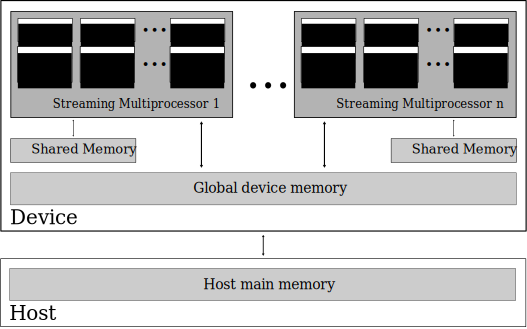
\includegraphics[width=\textwidth]{graphics/cuda-structure}
  \caption{CUDA GPU terminology: Host, devices, streaming
    multiprocessors and CUDA cores. The arrows show the possible path
    of data movement. The host can command movement of data to and
    from host memory and device memory. Kernel code is responsible for
    moving data between global memory, shared memory and registers.}
  \label{fig:gpu_terminology}
\end{figure*}

The architecture of NVIDIAs latest line of GPGPU devices is named
Kepler. The current Kepler based GPUs consists of up to 2880 CUDA
cores grouped into streaming multiprocessors of 192 cores each
\cite{nvidia2012keplerGK110}. At the HIPERFIT Research Center we have
access to a machine with two GeForce GTX 690 GPUs, each of which
contains two Kepler GK104 GPUs. The Kepler GK104 GPU is equipped with
1536 CUDA cores arranged into eight multiprocessors and shared between
all SMs is an L2 Cache (512 KB) and 2 GiB global memory
\cite{nvidia2012geforcegtx680}.

Figure \ref{fig:kepler_sm} shows the structure of a Kepler GK104
streaming multiprocessor. All 192 cores share the same register file
and 64 KB of additional memory which can be used both as L1 cache and
shared memory between for the CUDA cores of the SM. The amount of
memory used as cache and as shared memory is configurable.

\begin{figure}
  \centering
  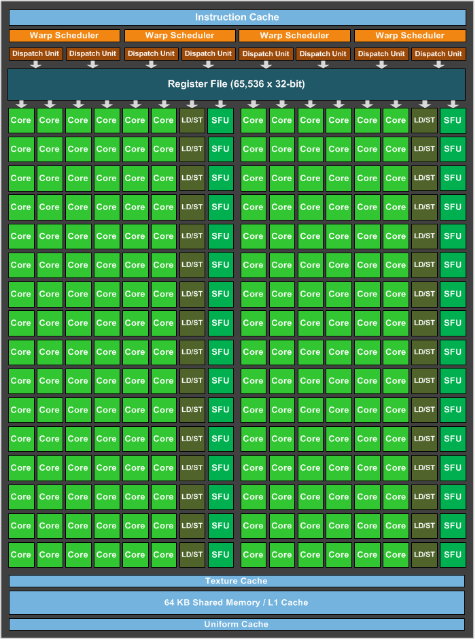
\includegraphics[width=0.8\textwidth]{graphics/nvidia_kepler_gk104_sm_cropped}
  \vspace{2mm}
  \caption{A diagram of a single streaming multiprocessor from a
    Kepler GK104 GPU. The illustration is borrowed from NVIDIAs GK104
    whitepaper \cite{nvidia2012geforcegtx680}, and a few irrelevant
    parts are cropped away..}
  \label{fig:kepler_sm}
\end{figure}

\section{GPU programming}
Since modern GPUs contains hundreds or thousands of cores, GPU
programs must be written such that their work can be executed
independently and in parallel on as many cores as possible. A single
thread of execution on a CUDA core is the smallest unit of work on a
GPU and programming a GPU is done by writing \textit{kernel programs}
or simply \textit{kernels}, which specifies the work done by a single
thread.

These threads are arranged into equal sized groups called
\textit{blocks} and blocks are arranged into a grid.  It is the task
of kernel program itself to find the subset of the data that it has
to work on. That is, all executions of the kernel receives exactly the
same arguments, but the kernel can query where it is located in its
block and where that block is located in the grid, to determine which
part of the input arrays to work on.

When executing a grid of CUDA blocks on a Kepler architecture GPU,
each block is assigned to a single SM (each SM can process several
blocks). Each block is partitioned into \textit{warps} which are
groups of 32 threads, which are scheduled on the 192 CUDA cores of the
streaming multiprocessor. % \todo{explain warp schedulers and why there
  % are 4 rather than 6 schedulers}

All threads in a \textit{warp} always executes exactly the same
instruction, this is called \textit{SIMD}, single instruction,
multiple data. Moreover, when warps are executed by a SM it can
execute two warps from the same block simultaneously, as each SM have
access to two schedulers and the register file can be used for both of
the two warps independently. This is called \textit{SIMT} (single
instruction, multiple thread) as two threads are executed on the same
processor simultaneously. Each streaming multiprocessor can be
assigned a certain number of warps, which it switches between
executing. This is useful for hiding latency endured by memory access
or data dependencies between instructions.

\subsection{Synchronization}
It is not uncommon that several threads has to interact, when they are
cooperating to solve a problem. In these cases synchronization
primitives are necessary to avoid race-conditions. In CUDA there are
two levels of inter-thread synchronization. A kernel can synchronize
with the rest of the threads in its block by calling the
\lstinline{__syncthreads} CUDA function. To synchronize across blocks,
the programmer has to split program into two independent kernels and
call them sequentially with a call to \lstinline{cudaDeviceSynchronize}
in between.

\subsection{Optimization considerations}
Determining how the grid of threads are partitioned into blocks are of
importance when optimizing for fast execution. There should at least
be as many blocks as there are streaming multiprocessor, to avoid
having a stalled processor. If blocks have to wait for synchronization
with other blocks it might also be beneficial to have more than one
block per SM.

The size of blocks should also be considered, as having enough
available warps can hide latency from memory transactions. Accessing
global memory can stall a streaming multiprocessor for 200-400 cycles,
where as local memory access only partakes a couple of cycles
\cite{nvidia2012cudaguide}. This is not the largest bottleneck though,
as GPUs are presently connected to the host through PCI Express ports
which have a throughput limit of a little under 8 GB/s (with PCI
Express 3.0). Accessing global memory on the device can be done at
192.3 GB/s, for the GeForce GTX 690 (and the double of that if you
count both of its GPUs).

We just argued for increasing block size, to make sure there are
enough warps, but it is not always good for efficiency to have large
blocks, as each streaming multiprocessor has a limited amount of
registers and local memory. All threads currently executed on a SM
shares the same register-file, and blocks are only assigned to a SM if
there are enough available registers for all of its threads. Thus, to
get optimal occupancy, blocks must be sized such that the size of the
register-file is divisible by the total amount of needed registers. An
occupancy calculator created by NVIDIA is available as a spreadsheet
on the NVIDIA
website\footnote{\url{http://developer.download.nvidia.com/compute/cuda/CUDA_Occupancy_calculator.xls}}.

\subsection{Memory access patterns}
Accessing global device memory is always done in segments of 32, 64 or
128 bytes, and these accesses must be aligned such that segments are
placed in physical device memory with a segment, starting on addresses
that are a multiple of the segment size
\cite{nvidia2012cudaguide}. When a warp gets executed, the memory
transaction of individual threads are coalesced such that the needed
memory can be fetched by a single memory transaction. To minimize the
number of memory transactions, it is thus important to write kernels,
such that nearby threads which are scheduled in the same warp, will
access memory in the same memory region. Previous architectures had
strict rules for how data accesses should be distributed. If
simultaneous operations on memory from a warp was out of sequence on
such a device, all the operations was performed as separate memory
transactions. The same would happen if accesses were not aligned
correctly. From Compute Capability 2.X and higher, the global L2 Cache
is used, such that out of order accesses can be coalesced into single
transactions and misalignments can be handled as long as they do not
cross 128 byte boundaries. If a segment of 32 bytes are accessed such
that this access overlap two physical 32-byte segments, the 64-byte
segment containing both of them are loaded from global memory instead.

These considerations are explained in detail in ``The CUDA C
Programming Guide'' by NVIDIA \cite[Section~5.3.2]{nvidia2012cudaguide}.

%%% Local Variables:
%%% mode: latex
%%% TeX-master: "master"
%%% End:
